\documentclass[a4paper]{article}

\setlength{\oddsidemargin}{-1in}
\addtolength{\oddsidemargin}{0.05 \paperwidth}
\setlength{\evensidemargin}{-1in}
\addtolength{\evensidemargin}{0.05 \paperwidth}
\setlength{\textwidth}{0.9 \paperwidth}

\setlength{\topmargin}{-0.75in}
\addtolength{\topmargin}{0.05 \paperheight}
\setlength{\textheight}{\paperheight}
\setlength{\headheight}{0in}
\setlength{\headsep}{0in}
\setlength{\footskip}{0in}

\setlength{\parskip}{0.3cm}
\setlength{\parindent}{0pt}

\usepackage[T1]{fontenc}
\usepackage[utf8]{inputenc}
\usepackage[german]{babel}
\usepackage{textcomp}

\usepackage[default,scale=1.5]{opensans}
\usepackage[scaled=1.4]{beramono}
\linespread{1.7}

\usepackage{url}
\usepackage{graphicx}
\usepackage{grid-system}
\usepackage{booktabs}


\usepackage{color}
\definecolor{freifunkpink}{RGB}{215,0,73}
\definecolor{freifunkyellow}{RGB}{255,191,0}
\definecolor{lightgrey}{RGB}{220,220,220}

\usepackage{enumitem}
\setlist[itemize]{leftmargin=*}

\begin{document}
\thispagestyle{empty}

\begin{center}
\Huge \textit{\textbf{\textcolor{freifunkpink}{Internet für Geflüchtete}}} \\
\vspace{0.6cm}
\large Freifunk ist ein regionales Mitmach-Netz für WLAN und Internet.\\
Hilf uns das Netz in Deiner Nachbarschaft auszubauen \\
und teile Dein Internet mit anderen Menschen!
\normalsize

\vspace{1.0cm}
\end{center}

{ \fontfamily{augie}\selectfont{\huge {}Liebe Nachbarn!}}
\vspace{0.5cm}

Freifunk Darmstadt ist eine lokale, nicht-kommerzielle Initiative von ehrenamtlich Aktiven mit dem Ziel, in Darmstadt und Umgebung ein \emph{offenes} und \emph{kostenlos} nutzbares WLAN-Netzwerk aufzubauen. Wir stellen Technik bereit, mit der \emph{jeder} seinen Internetzugang \emph{unkompliziert} mit anderen (z.B. auch den eigenen Gästen) teilen kann. Das Netz ist so aufgebaut, dass die rechtlichen Risiken für Betreiber minimal sind und das Heimnetz geschützt bleibt.

Die Flüchtlinge, die seit kurzem Eure Nachbarn sind, benötigen einen Internetzugang, um Kontakt mit ihrer Familie und ihrer alten Heimat zu halten und sich im Internet zu informieren. Ein internetfähiges Smartphone besitzen viele Geflüchtete bereits. Nach Ihrer Flucht können sich viele jedoch die vergleichsweise teuren Datentarife der Mobilfunkanbieter nicht leisten.

Zur Zeit unterstützen schon etwa 400 Menschen in Darmstadt und Umgebung Freifunk und teilen ihren Internetzugang. \emph{Hier in der Nähe der Unterkunft für Geflüchtete wird aber zur Zeit noch dringend ein Zugangspunkt benötigt.}

Du kannst helfen und selbst einen Router aufstellen. Dieser sogenannte Freifunkknoten leitet den Datenverkehr dann über die Freifunk-Server ins Internet. Dadurch kann der Datenverkehr Dritter nicht auf Deinen privaten Anschluss zurückgeführt werden. Wir unterstützen gerne bei der Installation und beantworten offene Fragen. \textbf{Bitte kontaktierte uns, wenn Du gerne helfen möchtest.}

\vspace{0.67cm}
\hspace{-0.24cm}
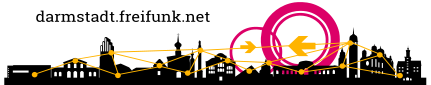
\includegraphics[width=0.965\paperwidth]{../images/footer_dark}

\newpage
\thispagestyle{empty}

\begin{Row}
  \begin{Cell}{5}
    \textbf{Werde ein Teil von Freifunk} \\
Freifunk-Netze sind Selbstmach-Netze. Auch Du kannst dazu beitragen, indem Du einen WLAN-Router mit der Freifunk-Software aufstellst und Deinen Internetzugang mit anderen teilst. Wenn viele mitmachen, entsteht ein flächendeckendes, freies WLAN-Netz.
  \end{Cell}
  \begin{Cell}{4}
    \textbf{Wir verstehen frei als:} \vspace*{-0.35cm}

		\begin{itemize}
			\setlength{\itemindent}{0.5em}
		  \item[\textcolor{freifunkpink}{\Large$\bullet$}] öffentlich \vspace*{-0.3cm}
		  \item[\textcolor{freifunkpink}{\Large$\bullet$}] anonym zugänglich \vspace*{-0.3cm}
		  \item[\textcolor{freifunkpink}{\Large$\bullet$}] nicht kommerziell \vspace*{-0.3cm}
		  \item[\textcolor{freifunkpink}{\Large$\bullet$}] unzensiert \vspace*{-0.3cm}
		  \item[\textcolor{freifunkpink}{\Large$\bullet$}] gemeinschaftlich betrieben\vspace*{-0.3cm}
			\item[\textcolor{freifunkpink}{\Large$\bullet$}] dezentral organisiert\vspace*{-0.3cm}
		  \item[\textcolor{freifunkpink}{\Large$\bullet$}] unabhängig
		\end{itemize}
  \end{Cell}
\end{Row}

\vspace{1.5em}

\begin{Row}
  \begin{Cell}{5}
    \textbf{Unsere Ziele}\vspace*{-0.35cm}
		\begin{itemize}
			\setlength{\itemindent}{0.5em}
			\item[\textcolor{freifunkpink}{\Large$\bullet$}] Aufklärung und Sensibilisierung zum Thema Kommunikationsfreiheit\vspace*{-0.3cm}
			\item[\textcolor{freifunkpink}{\Large$\bullet$}] Verminderung der digitalen Spaltung\vspace*{-0.3cm}
			\item[\textcolor{freifunkpink}{\Large$\bullet$}] Ungehinderte Verbreitung von Wissen und Ressourcen\vspace*{-0.3cm}
			\item[\textcolor{freifunkpink}{\Large$\bullet$}] Menschen dazu befähigen, eigene Netze aufzubauen und zu betreiben\vspace*{-0.3cm}
			\item[\textcolor{freifunkpink}{\Large$\bullet$}] Vorhandene und neue Sozialstrukturen fördern und vernetzen\vspace*{-0.3cm}
		\end{itemize}
  \end{Cell}
\end{Row}


\begin{center}
	\vspace{.3cm}
	\hspace*{-0.05 \paperwidth}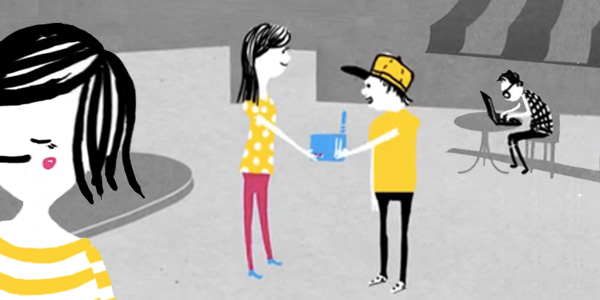
\includegraphics[width=\paperwidth]{../images/community_router}
\end{center}

Alle Informationen \& Kontakte findest Du auf \textbf{https://darmstadt.freifunk.net}.\\
Per Mail erreichst Du uns unter \textbf{info@darmstadt.freifunk.net}.

Informationen zu unseren wöchentlichen \textbf{offenen Treffen} finden sich auf unserer Webseite. Du bist herzlich eingeladen!

\end{document}
